\documentclass[conference]{IEEEtran}
\usepackage{amsmath,amssymb,booktabs,graphicx,balance}
\usepackage[hidelinks]{hyperref}
\usepackage{iftex}
\ifXeTeX
\usepackage{fontspec}
\setmainfont{texgyretermes-regular.otf}[BoldFont=texgyretermes-bold.otf,ItalicFont=texgyretermes-italic.otf,BoldItalicFont=texgyretermes-bolditalic.otf]
\setsansfont{texgyreheros-regular.otf}[BoldFont=texgyreheros-bold.otf,ItalicFont=texgyreheros-italic.otf]
\setmonofont{texgyrecursor-regular.otf}[BoldFont=texgyrecursor-bold.otf]
\fi
\hypersetup{pdftitle={When the Last Copy Leaves},pdfauthor={Anonymous working draft}}
\title{When the Last Copy Leaves:\\Recovering Graph Memory for Coding Agents}
\author{\IEEEauthorblockN{Anonymous working draft}}
\begin{document}
\maketitle
\begin{abstract}
A coding agent can recover repository context from a graph of files and the changes that linked them. After a restart, the reader may hold some event bodies in a write index, others in a bounded read cache, and a posting list that duplicates their addresses. We demonstrate a reader that remembers the event IDs absent from both volatile stores. When the last copy of a body leaves, its immutable membership list identifies which resident postings may need an update. A cardinality check certifies the reconstructed posting or triggers exact SQLite fallback. On six previously unmeasured repositories, 485 dense post-restart requests transferred 9,213 bytes at a 1\,KiB additional cache quota, versus 10,465 for count plus XOR and 11,531 for compressed full postings. The full-posting and maintained-exception readers tied at 4\,KiB. Visitors can evict either copy of an event, inspect real encoded packets, switch off notifications, and verify which reads are still required for the same answer.
\end{abstract}
\section{Introduction}
A coding agent investigating a source file often needs to reopen evidence from a previous session. Consider a developer who wants to know which neighboring files or tests changed together with a parsing module. One durable event per eligible Git change preserves the original grouping. Each participating file points to that event; a query uses the matching events to rank other files. The database can always answer from its journal. A small volatile index is useful when an agent returns to a file repeatedly or when another participant already keeps the relevant body in memory.

Which information should survive under pressure? A posting duplicates addresses already evident from resident event bodies. Replacing the posting with its count and XOR is sufficient to recover one missing ID, but several gaps generally require reading the authoritative list. Explicitly recording the missing addresses offers a different tradeoff: updates and evictions can become more expensive, while a future query may dispense with the posting read even when several bodies are absent.

The visitor can change cache placement, disable notifications and inspect actual packet bytes on a constructed graph. Separate views expose per-repository traffic, timing and replay on observed editor windows.

\section{Data model and exact baseline}
For a prefix of an append-only history let $e_j$ denote the distinct file IDs of its $j$th accepted event. The durable store holds one row per event, including its revision and varint-encoded members. A second table stores the sorted list $A_f=\{j:f\in e_j\}$ for each anchor $f$. A lookup returns up to eight other known files with largest
\begin{equation}
s(f,g)=\sum_{j\in A_f}{\bf 1}[g\in e_j].
\end{equation}
Recent file frequency over the preceding 32 source changes and then stable file ID resolve ties. An independent scorer builds the same top eight and their integer scores before the current change is appended. 

The hot write index gives each file ownership of its eight latest newly written events. An event remains visible from any participant while another owner still keeps it. A separate LRU read cache admits immutable event bodies and posting records, charging the packed key, length and payload for each. Keys are typed, so posting 7 and event 7 are distinct. The additional 1 or 4\,KiB quotas apply to this LRU; the write index, durable SQLite database and transient decoding buffers are accounted for separately. This common contract matters because storing more addresses necessarily leaves less room for bodies only inside a shared, charged budget.

At a read, first identify the resident events that truly contain the anchor. The write index can look them up by incidence. The complete two-tier implementation also inspects the bounded cached bodies. Define $R_f$ as the set of event IDs established by these two sources; the existence of a resident object alone says nothing about its participation in $f$. The ordinary exact-posting baseline encodes $A_f$ using the shortest of absolute varints, delta varints and a bitmap over its span. A further baseline stores the cardinality and XOR when shorter than a full list, recovering a single missing ID by cancellation. Both policies can cache event bodies under the same quota.

\section{Maintaining the missing addresses}
A retained exception record consists of a cardinality $n_f$ and an explicit set $E_f$ of IDs known to belong to $A_f$. When an exact list has just been resolved, the reader can initialize $E_f=A_f\setminus R_f$. The encoding pays a type byte, a varint for $n_f$ and, when nonempty, a compressed exact encoding of the exceptions. At admission the reader compares this representation with the full encoding and keeps the full list on a size tie. Future growth of a retained exception record is charged in the usual LRU replacement path.

\subsection{Exactness before work avoidance}
For a fixed committed prefix, suppose that $n_f=|A_f|$ and both $R_f$ and $E_f$ are subsets of $A_f$. Then
\begin{equation}
|E_f\cup R_f|=n_f\quad\Longleftrightarrow\quad E_f\cup R_f=A_f.
\end{equation}
The forward implication follows from inclusion and equal finite cardinalities; the reverse is immediate. An exception may become resident again. The union prevents double counting, so such overlap preserves correctness.  If membership evidence is incomplete, the left side is smaller and the reader falls back to the full posting in SQLite. Once all addresses are known, any unavailable bodies still have to be fetched. The method can avoid one posting read while requiring the very same body reads as its comparator.

Equation (2) requires positive membership witnesses and a cardinality from the same version. The store applies updates after source commits. Failed writes and duplicates must not increment $n_f$ twice.

\subsection{The moment of last eviction}
Suppose event $j$ leaves the read cache. While the write index still contains its body, $j$ remains available for all of its participants. Once the \emph{last} resident copy disappears, the evicted body itself supplies the list of affected files. For each of its participants with a resident exception record, insert $j$ into $E_f$ if needed. Files without a resident posting require no update. Eviction in the other direction is symmetric: if a new event displaces the last write-index owner but a read-cache copy survives, the insertion can be skipped.

The implementation records displaced read-cache bodies on a queue. Updating one retained posting changes its packed size and can evict another body. Draining the queue handles these cascades and checks current residency before recording a loss. An append has a small set of possible last owners, namely the oldest held event for each updated participant whose eight slots were full. The implementation rechecks those candidates after the append. It avoids a persistent file-to-record reverse index outside the quota. The queue and candidate list consume transient memory and the inspection of some resident bodies consumes CPU; both are reported explicitly.

A control retains the same exception encoding and performs the same cardinality test but skips loss notifications. It still returns exact results by reading the authoritative posting when necessary. Comparing it with the maintained variant isolates the value of knowing \emph{when} the encoded exceptions ceased to cover the resident complement. Even notifications caused by inserting a posting record itself matter: admission may evict one of the bodies that made the new record compact.
\section{What a visitor does}
\subsection{Control the residency of individual events}
The offline console initially displays eight illustrative changes involving \texttt{reader.py}. Each body has one hot-index copy and one read-cache copy. Visitors toggle either copy in any order, undo actions or repeat them with notifications disabled. The displayed byte strings for full postings, count plus XOR, and all 256 possible exception sets are generated by the production Python codecs, including the charged packed record size.

Evicting the first copy of event 13 leaves it in $R_f$. Losing its last copy adds the address to $E_f$. Evicting both copies of event 45 produces a second exception (Fig.~\ref{fig:app}). The query displays the necessary posting requests, missing bodies and ranked files. Disabling notifications forces a posting fallback for exactly the same answer. Restoring a copy creates overlap between the sets in (2).

\begin{figure}[t]\centering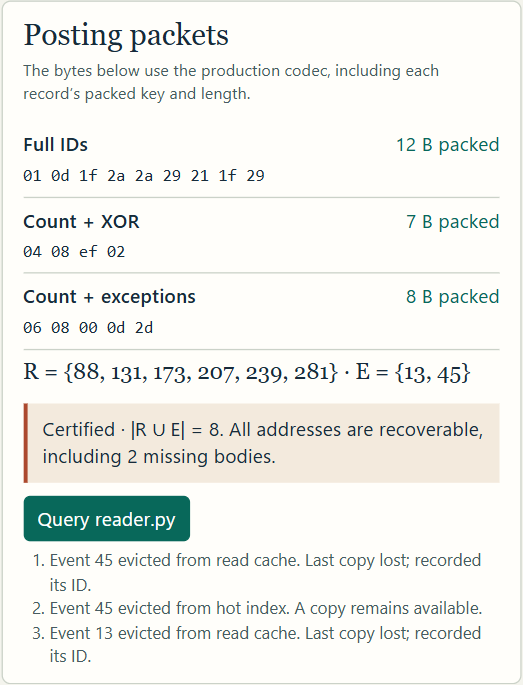
\includegraphics[width=.76\columnwidth]{lab.png}
\caption{Console after the last copies of two events have left. The exact address union remains certified. Hexadecimal record bytes come from the same encoders as the database runs.}\label{fig:app}
\end{figure}

Inspecting the constructed graph leaves placement intact. The trial view uses chronological SQLite runs with actual admissions and cascading evictions. Visitors select the cohort, schedule, quota and repository to compare posting and body bytes, SQL calls and multiple-gap certifications.

\subsection{Compare evidence rather than labels}
The dense histories were divided into a twelve-repository development and transfer group, a previous six-repository holdout already measured for XOR, and a fresh group of six repositories fixed for the present method. The evaluation keeps the same policy and budget on the fresh group, including a project with no sparse post-restart queries. We extracted Git commit and tree metadata only, independently verifying changed paths against raw tree objects. The new group contains 3,566 first-parent transitions across Alabaster, PyData Sphinx Theme, NumPy Financial, Tablib, Tomlkit and Jinja. Of those, 966 changes involved between two and 64 Python paths.

All policies reopen halfway through the eligible events. The dense schedule asks one hash-selected file query for each eligible commit following the first 64 source transitions. The sparse schedule starts halfway through source history and selects eligible commits by a fixed hash residue. Readers see the same ordered questions and earlier writes. The endpoint of interest is logical SQLite BLOB payload returned across that program boundary. Physical page traffic and bidirectional network exchanges require separate measurement.

\begin{table}[t]\centering
\caption{Dense payloads from SQLite after restart at 1 KiB. The two exception methods share the same packet format.}\label{tab:main}
\begin{tabular}{lrrrr}\toprule
Panel (queries) & Full & XOR & No notify & Maintained\\\midrule
Prior 12 (2,063) & 123,019 & 115,945 & 118,988 & 109,005\\
Prior 6 (721) & 21,957 & 20,055 & 22,941 & 17,177\\
New 6 (485) & 11,531 & 10,465 & 16,991 & 9,213\\\bottomrule
\end{tabular}
\end{table}

\section{Measured effects and controls}
At the primary 1\,KiB point, maintained exceptions saved 6,940 bytes relative to XOR on the twelve older dense streams. Ten repositories improved and two tied. In the previous six-project holdout four improved and two tied. On the new panel, the saving against XOR was 1,252 bytes (12.0\%) or 2,318 bytes (20.1\%) against compressed full postings. Three repositories improved and three tied against either comparator. Tomlkit contributed 972 bytes of the saving against XOR, followed by Jinja with 183 and Tablib with 97 (Fig.~\ref{fig:projects}). Repeated queries in one project can share the same retained objects; the 485 queries are not 485 independent repositories.

\begin{figure}[t]\centering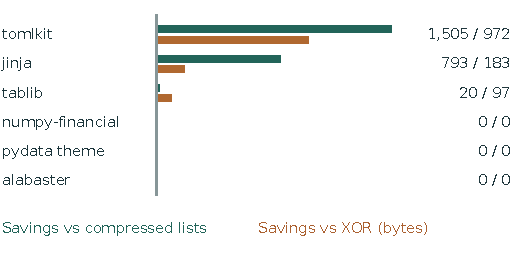
\includegraphics[width=\columnwidth]{projects.pdf}
\caption{Savings on each fresh repository at 1 KiB, in dense traffic. The top bar of each pair compares against compressed full postings and the lower bar against XOR. Three projects tie in both contrasts.}\label{fig:projects}
\end{figure}

For the new dense group the maintained reader returned 5,085 posting bytes and 4,128 body bytes. It issued 374 read calls and certified a list with two or more missing bodies 14 times. It inserted 1,003 additional exception IDs during maintenance. The earlier twelve projects produced 45 multiple-gap certifications at the same budget. The no-notification control used 16,991 bytes in the new dense group, exceeding the three alternatives in Table~\ref{tab:main}. Realizing the advantage of the representation required processing last-copy events.

At 4\,KiB on the new dense group, both the maintained and compressed full readers transferred 4,322 bytes while XOR transferred 5,678. On the 45 new sparse queries, full and maintained both returned 2,525 bytes at either quota. Enough space for full postings, or too little repeated demand for a smaller representation, can remove the measured benefit. 

\subsection{Stronger posting baselines}
A shorter representation of \emph{all} event IDs is a plausible alternative explanation. To test it we added binary interpolative coding, Elias--Fano and serialized Roaring bitmaps to the original full-posting encoder. Each list can choose the smallest available exact format, and the exception method can also use any of them for its residual addresses. On the same 485 queries at 1\,KiB, the full-list suite required 11,372 bytes and maintained exceptions required 9,201, saving 19.09\%. At 4\,KiB both required 4,322. This comparison addresses encoding quality for these measured lists, while a broader state-of-the-art claim would require comparison with other systems under matching memory and durability contracts.

\begin{table}[t]\centering
\caption{Control for source payload and CPU on 485 new queries. Time is the median across three local technical blocks.}\label{tab:cpu}
\begin{tabular}{lrrrr}\toprule
 & \multicolumn{2}{c}{1 KiB} & \multicolumn{2}{c}{4 KiB}\\
Method & Bytes & ms & Bytes & ms\\\midrule
Append-efficient full & 11,646 & 41.53 & 4,322 & 38.94\\
Count + XOR & 10,465 & 57.38 & 5,678 & 64.48\\
Two-tier exceptions & 9,213 & 71.06 & 4,322 & 67.99\\
Hot-only, trusted & 10,863 & 52.42 & 4,322 & 51.37\\\bottomrule
\end{tabular}
\end{table}

\subsection{The locality and price of notifications}
The CPU comparison exposes work omitted from SQLite payload accounting. At 1\,KiB the two-tier method scanned 110,897 resident bytes during query-time validation on the new dense group. A more append-efficient full-posting control used 11,646 payload bytes and completed the timed reads plus cache maintenance in 41.53\,ms. Two-tier exceptions took 71.06\,ms on the same workload (Table~\ref{tab:cpu}). The hot-only variant defines the complement relative only to the existing write index. Under reliable local notification delivery it avoids consulting the additional read-cache bodies to certify coverage. Its intermediate cost, 10,863 bytes and 52.42\,ms, illustrates another point in the time--traffic tradeoff. A separate five-block comparison reused encoded postings and specialized complete resident hits. Under guaranteed notification delivery an exception format omitting the redundant count used 9,187 bytes and 38.16\,ms on the new six, versus 11,646 and 38.75\,ms for reused full postings. Retaining only the shared hot write index was faster at 35.39\,ms but transferred 14,918 bytes. Across the two six-project panels the paired totals were 26,122 bytes and 91.43\,ms versus 33,837 and 94.60\,ms. These are small local timing differences under a stronger delivery assumption.

Bidirectional request framing also changes the comparison. In a loopback protocol serving the same 485 dense requests, maintained exceptions used 16,533 application bytes and 374 remote calls at 1\,KiB, count plus XOR used 17,919 and 386, and the full format used 20,115 and 412. At 4\,KiB, the maintained and full methods tied at 9,146 bytes and 281 calls. Server-side ranking changes these charges again depending on synchronization of the tie-breaking prior.

\subsection{A check on observed agent actions}
The Git schedule is an artificial workload. We performed a separate replay on 108 published SWE-agent sessions comprising 54 tasks. Actual editor windows supply the path and line coordinates. After half of a session's windows, a modeled graph query uses the first displayed 16-line block as an anchor before recording the jointly observed blocks. This yields 436 post-restart queries. Full postings, XOR and maintained exceptions each cost 1,668 bytes at 1\,KiB. With four-line blocks and a deliberately tight 256-byte quota, their totals were 7,798, 7,650 and 7,636 bytes. All primary 16-line regimes tied. The trace replay tests a modeled memory operation on real actions; it provides no evidence for increased patch success.
\section{Relation to prior work}
Mining source changes for file recommendations predates this system~\cite{rose,moonen}. It gives us a simple, inspectable graph whose exact query can be recomputed.  TAPE exposes temporal graph memory for personal agents~\cite{tape}. Our experiment isolates representation and recovery for a fixed exact access pattern, rather than comparing systems with different extraction, relevance or model-generation policies.

WebGraph compresses adjacency lists by exploiting similarity to another list and encoding the residual information~\cite{webgraph}. That work motivates a natural question: relative to \emph{which} reference is an adjacency list inexpensive to encode? In this demonstration the reference is the union supported by the current resident bodies. Its contents change under cache pressure and can differ for each anchor even within the same query stream. The raw body supplies its participants exactly at the point where the final copy departs. The resulting maintenance rule and independent comparison against modern full-list encodings are central to the measured claim.

Noria studies partially materialized dataflow and reconstructs state in response to demand~\cite{noria}. Here the durable filelist and bodies remain complete and the optional compact object sits above that exact source. We exploit the fact that one graph object supplies verifiable incidences for several postings, which also makes updating the last copy more expensive than simply discarding an object. Algebraic recovery by XOR is classical in set reconciliation~\cite{iblt}. Remembering explicit residual IDs can handle more missing entries but incurs different update and representation costs. The observed contribution is thus a specific eviction-aware policy and the evidence for its useful operating conditions. It is not a claim to have invented residual adjacency coding, partial materialization or set reconciliation.

\section{Correctness and artifact use}
The evaluator checks complete sorted answers, including zero-score ties. Across 48 workload--repository cases there were 3,563 post-restart queries and 28,504 rank comparisons for the two limits and four policies. An additional check directly compared each reconstructed incidence sequence with the authoritative prefix for both exception variants. The independent finite-state test enumerated 15,625 combinations and 37,500 transfers between resident and exception sets. A second physical SQLite test forced five body losses, verified five identical-length member payloads (15 bytes total), and observed zero posting calls with notifications versus one without. This isolates reconstruction from any reduction in the cost of reading the bodies.

Failure-oriented tests also cover updates during eviction. The measured implementation detected 217 secondary evictions triggered by exception updates, checked 5,778 resident posting records and compared 2,032 ranks. Four rolled-back writes, eleven suppressed duplicates, eleven conflicting repeats and three cold reopenings exercised transaction and version boundaries. The source archive must remain available and append-only for these identities. A deployment that permits deletion, file-ID recycling or asynchronous invalidation would need additional version and reliability mechanisms. A checksum alone cannot preserve the subset invariant across a version change.

The offline registry ships with the encoders, SQLite replays and independent checks.

\balance
\section{Conclusion}
An explicit record of missing event addresses makes exact reconstruction possible across several simultaneous cache gaps. In the evaluated low-capacity dense settings, reliable last-copy notifications reduced the amount of data returned by SQLite relative to compressed full postings and XOR. The same policy tied full postings on larger and shorter workloads and added CPU work in the measured two-tier implementation. Inspecting those limits alongside successful cases gives the visitor a concrete criterion for deciding which representation to use.

\section*{Acknowledgment}
OpenAI Codex assisted with implementation, analysis and drafting. Anonymous working draft.

\begin{thebibliography}{6}
\bibitem{rose} T. Zimmermann, P. Weisgerber, S. Diehl, and A. Zeller, “Mining version histories to guide software changes,” in \emph{ICSE}, 2004, pp. 563--572. \href{https://doi.org/10.1109/ICSE.2004.1317478}{doi:10.1109/ICSE.2004.1317478}.
\bibitem{moonen} L. Moonen, S. Di Alesio, D. Binkley, and T. Rolfsnes, “Practical guidelines for change recommendation using association rule mining,” in \emph{ASE}, 2016, pp. 732--743. \href{https://doi.org/10.1145/2970276.2970327}{doi:10.1145/2970276.2970327}.
\bibitem{tape} C. Luo, Q. Liu, W. Zhang, and Y. Gao, “TAPE: A temporal graph-based memory system for personal LLM agents,” in \emph{ICDE}, 2026, pp. 4168--4171. \href{https://doi.org/10.1109/ICDE65706.2026.00318}{doi:10.1109/ICDE65706.2026.00318}.
\bibitem{webgraph} P. Boldi and S. Vigna, “The WebGraph framework I: Compression techniques,” in \emph{WWW}, 2004, pp. 595--602. \href{https://vigna.di.unimi.it/ftp/papers/WebGraphI.pdf}{Author copy}.
\bibitem{noria} J. Gjengset et al., “Noria: Dynamic, partially-stateful data-flow for high-performance web applications,” in \emph{OSDI}, 2018, pp. 213--231. \href{https://www.usenix.org/conference/osdi18/presentation/gjengset}{USENIX}.
\bibitem{iblt} M. T. Goodrich and M. Mitzenmacher, “Invertible Bloom lookup tables,” \emph{arXiv:1101.2245}, 2011, revised 2015. \href{https://arxiv.org/abs/1101.2245}{arXiv}.
\end{thebibliography}
\end{document}
